% $  Id: validation.tex  $
% !TEX root = main.tex


%%
\section{Validation}
\label{sec:validation}

This section provides empirical experimentation of the \ac{ML} techniques introduced in the previous 
section. Two application for pattern recognition were selected to execute each of the techniques. The 
first application uses existing housing system data to learn and predict market prices. The second 
application, uses pattern recognition for the identification of objects (flowers) in an image.

%%%%
\subsection{Execution Environment}

The first experiment used data provided by Google's Machine Learning Crash 
course~\cite{mlchrome18}. The experiment was run using TensorFlow directly on the Google 
Chrome browser using google's collaboration platform. 
%Nonetheless, it is possible to execute the program offline which requires the user to set up a local Datalab environment by installing Docker~\cite{docker18}.   
The second experiment was developed using TensorFlow version 1.0 running in a Jupiter 
Notebook with python 3 accessed through Anaconda. 
Both experiments were run on a 2013 Intel Core i5 MacBook Air with macOS Sierra version 10.12.6.

%%%%
\subsection{Learning with Linear Regression}

For the first experiment resources and learning material were taken from Google’s Artificial 
Intelligence course. The course provides knowledge for beginners and experts, as well as practice 
material and online classes. The experiments uses data from 1990’s housing system in California. 
Based on this data, we want to build a model capable of predicting median house value at the 
granularity of city blocks based on a specific feature from the available data set (\eg median age, 
median value)~\cite{mlchrome18}. 

When starting a \ac{ML} project, the most important part is to understand the available data.
Taking advantage from data insights it is possible to obtain a more accurate model. The housing data 
(\ie \emph{data frame}) used in this experiment is composed of nine features,\footnote{\url{https://storage.googleapis.com/mledu-datasets/california_housing_train.csv}} namely: 
\begin{enumerate*}[label=(\arabic*)]
\item \tensorcode{longitude},
\item \tensorcode{latitude},
\item median age (\tensorcode{housing_median_age}),	
\item total number of rooms (\tensorcode{total_rooms}),	
\item total number of bedrooms (\tensorcode{total_bedrooms}),
\item \tensorcode{population},	
\item \tensorcode{households},
\item median income (\tensorcode{median_income}), and
\item	median house value (\tensorcode{median_house_value}).
\end{enumerate*}
These features are classified according to their data type --that is, categorical (\eg text), or numeric 
(\eg number, integer, float). Features describe how the model should use raw input data from a 
features dictionary. Raw data, in TensorFlow, is processed through \emph{Estimators}, exposed as 
the high-level API of the language~\cite{tensor18}. \fref{lst:feature-configuration} shows the definition 
of a desired input feature, and its classification as a numeric feature, using the TensorFlow high-level 
API.

\begin{tensorflow}[
	label={lst:feature-configuration},
	caption={Feature definition and classification}]
 # input feature is designated
 my_feature = california_housing_dataframe[["total_rooms"]]

 # A numeric feature column for total_rooms is configured.
 feature_columns = [tf.feature_column.numeric_column("total_rooms")]
\end{tensorflow}

The goal for this experiment is to estimate the median house value based on historic data, available to 
users. These characteristics suggest to use the linear regression model for the estimation.
As explained in \fref{sec:linear-regression}, we create the linear regression model 
(\fref{ln:linear-model}) based on the gradient  decent (Lines \ref{ln:gradient-init}-\ref{ln:gradient-end}) as 
shown in \fref{lst:lrm}.

\begin{tensorflow}[numbers=left,
	label={lst:lrm},
	caption={Generation of the linear regression model}]
 #Gradient Descent declaration
 my_optimizer=tf.train.GradientDescentOptimizer(learning_rate=0.0000001) ` \label{ln:gradient-init} `
 my_optimizer = tf.contrib.estimator.clip_gradients_by_norm(my_optimizer, 5.0) 
 ` \label{ln:gradient-end} `

 #Include the feature columns and optimizer in the configuration of the  linear regression model.
 #Learning rate is set to  0.0000001 for the Gradient Descent
 linear_regressor = tf.estimator.LinearRegressor(feature_columns=feature_columns, optimizer=my_optimizer) ` \label{ln:linear-model} `
\end{tensorflow}

As with other \ac{ML} techniques, in order to make a prediction, the model needs to be trained using 
available data. In order to train the model, it is necessary to batch, preprocess, and shuffle the data. 
This is to assure that the model will not be trained on biased data. 
Training a linear regression model requires a function (\tensorcode{input_fn} in 
\fref{lst:training}) characterized by the feature to make the prediction (\tensorcode{my_feature}), as 
well as the targets (of the estimation). Finally developers are required to define the number of steps 
in which the model will be trained.

\fref{lst:training} shows the training definition for the the housing system data. in this example we 
train the model for 100 steps, using as input feature \tensorcode{total_rooms}, defined in 
\fref{lst:feature-configuration}. 

\begin{tensorflow}[
	label={lst:training},
	caption={Model training}]
 _ = linear_regressor.train(
    input_fn = lambda:my_input_fn(my_feature, targets),
    steps=100
 )
\end{tensorflow}

The decision of using 100 training steps the outcome of the model fitting process, where developers 
are required to fine tune the model parameters to assure accurate predictions. During training, it is 
required to measure the effectiveness of the model. If prediction errors are identified, for example 
using the least square error, it is required to adjust the model \emph{hyperparameters}. That is, 
modifying the batch size, learning rate, or number of steps, to find a good fit with low prediction error. 

During the fitness process, the model should be fit to foster \emph{generalization}. 
Generalization refers to the model’s ability to adapt to new, previously unseen data, drawn from the 
same distribution as the one used to create the model.  Generalization allows for all training examples 
to be correctly classified. If the model works well with predictions on the test set and the data set, then 
this is a good indicator about how the model is going to perform when dealing with new unseen data.  


%%%%
\subsection{Learning with Neural Networks}

The project regarding Neural Networks was developed using content provided by TensorFlow's website~\cite{tensor18}. The goal was to classify flowers based on a dataset containing plant measurements such as sepal length, sepal width, petal length and petal width. In more detail, the Model had to classify the data into one of three Iris flowers: Iris Setosa, Iris Versicolor and Iris Virginica. 
As mentioned before in this document, models are not able to directly receive objects as information, thus the first step towards completion was setting a representation of each flower for the model to understand. 

\begin{figure}[htbp]
  \centering
  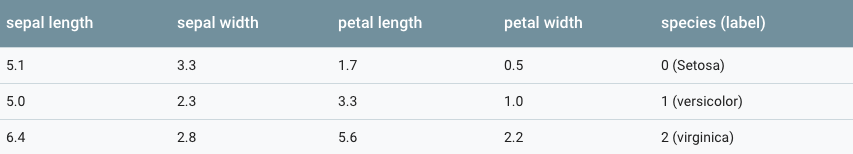
\includegraphics[width=\textwidth]{images/table}
  \caption{Data representation used for modeling (taken from~\cite{tensor18})}
  \label{fig: rep}
\end{figure}

Although TensorFlow Linear Classifier Estimator was also applicable for this problem, it was required to use the DNNClassifier to perform multi-class classification~\cite{tensor18}. Because the information volume was not very large it was appropriate to develop a four layer model. The two outer layers correspond to the indispensable input and output layers, as a result  two hidden layers remained in the net. Specifically entering into details concerning the Neural Network development, the DNNClassifier  provided accesible tools to model the structure of the net.

\begin{tensorflow}[caption={ads}]
# Net contains 2 hidden layers with 10 nodes each.
classifier = tf.estimator.DNNClassifier(
    feature_columns=my_feature_columns,
    hidden_units=[10, 10],
# The model must choose between 3 classes which represent each flower.
    n_classes=3)
\end{tensorflow}

Continuing, as implemented in the project above, the first steps to achieve a good model was creating the input functions, and defining the model's feature columns. 

\begin{tensorflow}[caption={ads}]
#Input function definition
def input_evaluation_set():
    features = {'SepalLength': np.array([6.7, 5.3, 4.4]),
                'SepalWidth':  np.array([3.4., 4.2, 3.1]),
                'PetalLength': np.array([5.6, 3.3, 4.8]),
                'PetalWidth':  np.array([2.2, 1.0, 2.8])}
    labels = np.array([3, 1])
    return features, labels
\end{tensorflow}

Interestingly the results obtained by the model's classification where expected to sum up to one. In other words, the model was designed to respond to each input by deciding in which proportion the data corresponds to one of the three available flowers. 

\begin{enumerate}
 \item 0.08 for Iris Setosa
 \item 0.02 for Iris Versicolor
 \item 0.90 for Iris Virginica
\end{enumerate}

From the above example it is possible to conclude that the model determined a 90 percent probability of the data corresponding to an Iris Virginica.   Following this, the closing section of the process was developed in a similar manner to the first project. Namely, training the model and evaluating proceeded. Just like in the first  application, training was implemented using the Estimators train method. 

%%%%
\subsection{Experiments Analysis}

For both, the Housing and Flower problems, models were trained and predictions were made. When working with information such as the California Housing system, where there is a large amount of data classified in different ways, it was possible to determine empirically that Linear Regression supervised Machine Learning was the most appropriate way to recover a certain trait present in the data. This statement is drawn from the fact that no previous outcome was determined for each information used in the model, thus adjusting Hyperparameters was the only resource available for the user to shape the model.  From here evaluations were made concluding that indeed Linear Regression models present useful solutions while keeping the process accessible and simple for users that are starting to work with \ac{ML}.  On the other hand information accesible for the second project was different resulting in the implementation of a distinct form of \ac{ML}. In this case there was a set of characteristics in which information was supposed to fit in, based on this a Neural Network approach was more feasible. The complexity of the model's input reflected how the Network was modeled and how deep the layers were. Additionally, thanks to probability provided by the model, classifying data becomes a process in which results over time sharpen the classification precision. 


Practitioners using \ac{ML} for a particular project, should only be concerned with the high-level API, providing out-of-the-box estimators appropriate to the specific \ac{ML} technique to use.

%%%%
%\subsection{Threads to Validity}



\endinput



